%%%%%%%%%%%%%%%%%%%%%%%%%%%%%%%%%%%%%%%%%
% Masters/Doctoral Thesis 
% LaTeX Template
% Version 1.43 (11/01/2015)
%
% This template has been downloaded from:
% http://www.LaTeXTemplates.com
%
% Original authors:
% André Carvalheira 
% http://users.ecs.soton.ac.uk/srg/softwaretools/document/templates/
% and
% Sunil Patel
% http://www.sunilpatel.co.uk/thesis-template/
%
% License:
% CC BY-NC-SA 3.0 (http://creativecommons.org/licenses/by-nc-sa/3.0/)
%
% Note:
% Make sure to edit document variables in the Thesis.cls file
%
%%%%%%%%%%%%%%%%%%%%%%%%%%%%%%%%%%%%%%%%%

%----------------------------------------------------------------------------------------
%	PACKAGES AND OTHER DOCUMENT CONFIGURATIONS
%----------------------------------------------------------------------------------------

\documentclass[11pt, oneside]{Thesis} % The default font size and one-sided printing (no margin offsets)

\graphicspath{{Pictures/}} % Specifies the directory where pictures are stored

\usepackage[square, numbers, comma, sort&compress]{natbib} % Use the natbib reference package - read up on this to edit the reference style; if you want text (e.g. Smith et al., 2012) for the in-text references (instead of numbers), remove 'numbers' 
\usepackage{booktabs}
\usepackage{hyperref}
\hypersetup{urlcolor=blue, colorlinks=true} % Colors hyperlinks in blue - change to black if annoying
\title{\ttitle} % Defines the thesis title - don't touch this

\begin{document}

\frontmatter % Use roman page numbering style (i, ii, iii, iv...) for the pre-content pages

\setstretch{1.3} % Line spacing of 1.3

% Define the page headers using the FancyHdr package and set up for one-sided printing
\fancyhead{} % Clears all page headers and footers
\rhead{\thepage} % Sets the right side header to show the page number
\lhead{} % Clears the left side page header

\pagestyle{fancy} % Finally, use the "fancy" page style to implement the FancyHdr headers

\newcommand{\HRule}{\rule{\linewidth}{0.5mm}} % New command to make the lines in the title page

% PDF meta-data
\hypersetup{pdftitle={\ttitle}}
\hypersetup{pdfsubject=\subjectname}
\hypersetup{pdfauthor=\authornames}
\hypersetup{pdfkeywords=\keywordnames}

%----------------------------------------------------------------------------------------
%	TITLE PAGE
%----------------------------------------------------------------------------------------

\begin{titlepage}
\begin{center}

\begin{figure}[htbp]
\centering

\includegraphics[width=0.3\textwidth]{Pictures/fctuc.png}
\end{figure}

\textsc{{\facname} of the {\univname}}\\[1.5cm] % University name
\textsc{\Large Master Thesis}\\[1cm] % Thesis type

\HRule \\[1cm] % Horizontal line
{\huge \bfseries \ttitle}\\[0.4cm] % Thesis title
\HRule \\[1.5cm] % Horizontal line
 
\begin{center} \large
\emph{by}\\
\href{}{\authornames}\\[1.5cm] % Author name - remove the \href bracket to remove the link

\emph{Under the supervision of} \\[0.5cm]
{\supname}\\[3cm] % Supervisor name - remove the \href bracket to remove the link  
\end{center}
 
\large \textit{A thesis submitted in fulfilment of the requirements\\ for the degree of {\degreename} of Science of Biomedical Engineering}\\[2cm] % University requirement text

 
{\large \today} % Date
%\includegraphics{Logo} % University/department logo - uncomment to place it
 
\vfill
\end{center}

\end{titlepage}

%\addtocontents{toc}{\vspace{1em}} % Add a gap in the Contents, for aesthetics
\pagestyle{empty} % No headers or footers for the following pages


\clearpage


%----------------------------------------------------------------------------------------
%	LOGOS
%----------------------------------------------------------------------------------------

\begin{center}
This work was developed in collaboration with:\\[2cm]

\begin{figure}[htbp]
\centering

\includegraphics[width=0.78\textwidth]{Pictures/exa.png}\\[0.5cm]
\end{figure}

\textsc{\Large \bfseries Exatronic Insight Innovation | Aveiro, Portugal }\\[2cm]

 

\begin{figure}[htbp]
\centering

\includegraphics[width=0.78\textwidth]{Pictures/fctuc_logo.jpg} \\[0.5cm]
\end{figure} 

\textsc{\Large \bfseries Electronics and Instrumentation Group (GEI) \\ Department of Physics, University of Coimbra \\[0.2cm] Coimbra, Portugal }\\[2cm]






\end{center}



\clearpage
%----------------------------------------------------------------------------------------
%	direitos de autor
%----------------------------------------------------------------------------------------



\null
\vfill

Esta cópia da tese é fornecida na condição de que quem a consulta reconhece
que os direitos de autor são pertença do autor da tese e que nenhuma citação ou
informação obtida a partir dela pode ser publicada sem a referência apropriada.

This copy of the thesis has been supplied on condition that anyone who
consults it is understood to recognize that its copyright rests with its author and that
no quotation from the thesis and no information derived from it may be published
without proper acknowledgement

\clearpage
%----------------------------------------------------------------------------------------
%	QUOTATION PAGE
%----------------------------------------------------------------------------------------


\null\vfill % Add some space to move the quote down the page a bit

\textit{``Thanks to my solid academic training, today I can write hundreds of words on virtually any topic without possessing a shred of information, which is how I got a good job in journalism."}

\begin{flushright}
Dave Barry
\end{flushright}

\vfill\vfill\vfill\vfill\vfill\vfill\null % Add some space at the bottom to position the quote just right

\clearpage % Start a new page

%----------------------------------------------------------------------------------------
%	ABSTRACT PAGE
%----------------------------------------------------------------------------------------
\thispagestyle{plain}
\addtotoc{Abstract} % Add the "Abstract" page entry to the Contents

\begin{center}
 {\huge{\textit{Abstract}} \par}
  \bigskip
\end{center}

%\abstract{%\addtocontents{toc}{\vspace{1em}} % Add a gap in the Contents, for aesthetics


\textit{\Large 1st - The problem}

NEED - At the same time we have an increase quality of life and consequently on life expectancy and on aging population. More diseases. Cardiovascular diseases are the number one worldwide cause of death. No Infraestructure

APPROACH - To meet the need (growing number of diseases) evidenced by this population medical devices sector is developing solutions with integrated electronics in order to improve quality of life in all periods of life and preferred living environment. This is called Ambient Assisted Living (AAL). area and integrated (módulos)

"Ambient Assisted Living" (AAL) are concepts, products and services which combine new technologies and the social environment in order to improve quality of life in all periods of life and preferred living environment

BENEFITS - Thus, increasingly arise  of portable solutions allow quick monitorization of vital parameters with the purpose of diagnosing diseases earlier and prevent emergency situations.

This project has as main goal the development hardware, firmware and software for a blood pressure measurement device.

\textit{\Large 2nd}

WHAT - This thesis details the development of a  blood pressure device prototype with wireless communication of their readings that will be part of a multi-module device with oxymetery, ECG, etc .
 
HOW - The work includes the creation schmetics and a Printed Circuit Board (PCB) which integrate all the selected components for this device.
The system was programmed using an Atmel debugger, AVR Dragon, and a development board with a microcontroller (MCU), ATxmega 384C3, for whom all the firmware was developed

\textit{\Large{3rd}}

The main goal was to have a fiable device. Even thought factors like electric consumption of all the components were studied having in mind a a portable prototype.

System tests
Interface (HMI) - web/Android
How did you stored that? 

\null
\vfill

\textbf{\emph{Keywords:}} \textit{Blood Pressure, Medical Devices, Ambient Assisted Living
(AAL), Internet of Things (IoT), ATmega2560/AVR Dragon, Bluetooth, Wireless Communication, Printed Circuit Board (PCB), ATxmega 384C3, Hardware, Altium Designer, Firmware, C Language, Signal Aquisition, C Language}

\clearpage % Start a new page

%----------------------------------------------------------------------------------------
%	RESUMO PAGE
%----------------------------------------------------------------------------------------
\thispagestyle{plain}
\addtotoc{Resumo} % Add the "Resumo" page entry to the Contents

\begin{center}
 {\huge{\textit{Resumo}} \par}
  \bigskip
\end{center}

Currently, Portugal displays indicators to be an aging population. In this light, the medical devices sector has been developing solutions~\cite{joao} that try to meet the needs evidenced by this population. Thus, increasingly arise mobile solutions such as solutions for monitoring vital parameters with the purpose of diagnosing diseases earlier and prevent emergency situations. These devices are part of the Ambient Assisted Living area~\cite{jose}.

The Exa4Life is also very attentive to this market sector and the Ambient Assisted Living solutions. As such, you want to see the emergence of solutions with electronic able to monitor vital parameters in a simple way so they can be used by the target audience in their preferred environment.

It is intended, then the students to develop a prototype device which is a 7medidor blood pressure with wireless communication of their readings.\ldots
%}

\null
\vfill


\textbf{Palavras-Chave:} \textit{Pressão Arterial, Dispositivos Médicos, Ambient Assisted
Living (AAL), Bluetooth, Comunicação Wireless, ATmega2560/AVR Dragon, Printed Circuit Board (PCB), ATxmega 384C3, Hardware, Altium
Designer, Firmware, Linguagem C, Aquisição de Sinal, Linguagem C}

\clearpage % Start a new page

%----------------------------------------------------------------------------------------
%	ACKNOWLEDGEMENTS
%----------------------------------------------------------------------------------------
\thispagestyle{plain}
\setstretch{1.3} % Reset the line-spacing to 1.3 for body text (if it has changed)

\addtotoc{Acknowledgements} % Add the "Resumo" page entry to the Contents

\begin{center}
 {\huge{\textit{Acknowledgements}} \par}
  \bigskip
\end{center}

Thanks!

\clearpage % Start a new page

%----------------------------------------------------------------------------------------
%	LIST OF CONTENTS/FIGURES/TABLES PAGES
%----------------------------------------------------------------------------------------

\pagestyle{fancy} % The page style headers have been "empty" all this time, now use the "fancy" headers as defined before to bring them back

\lhead{\emph{Contents}} % Set the left side page header to "Contents"
\tableofcontents % Write out the Table of Contents

\lhead{\emph{List of Figures}} % Set the left side page header to "List of Figures"
\listoffigures % Write out the List of Figures

\lhead{\emph{List of Tables}} % Set the left side page header to "List of Tables"
\listoftables % Write out the List of Tables

%----------------------------------------------------------------------------------------
%	ABBREVIATIONS
%----------------------------------------------------------------------------------------

\clearpage % Start a new page

\setstretch{1.5} % Set the line spacing to 1.5, this makes the following tables easier to read

\lhead{\emph{Abbreviations}} % Set the left side page header to "Abbreviations"
\listofsymbols{ll} % Include a list of Abbreviations (a table of two columns)
{
\textbf{LAH} & \textbf{L}ist \textbf{A}bbreviations \textbf{H}ere \\
%\textbf{Acronym} & \textbf{W}hat (it) \textbf{S}tands \textbf{F}or \\
}

%----------------------------------------------------------------------------------------
%	PHYSICAL CONSTANTS/OTHER DEFINITIONS
%----------------------------------------------------------------------------------------

\clearpage % Start a new page

\lhead{\emph{Physical Constants}} % Set the left side page header to "Physical Constants"

\listofconstants{lrcl} % Include a list of Physical Constants (a four column table)
{
Speed of Light & $c$ & $=$ & $2.997\ 924\ 58\times10^{8}\ \mbox{ms}^{-\mbox{s}}$ (exact)\\
% Constant Name & Symbol & = & Constant Value (with units) \\
}

%----------------------------------------------------------------------------------------
%	SYMBOLS
%----------------------------------------------------------------------------------------

\clearpage % Start a new page

\lhead{\emph{Symbols}} % Set the left side page header to "Symbols"

\listofnomenclature{lll} % Include a list of Symbols (a three column table)
{
$a$ & distance & m \\
$P$ & power & W (Js$^{-1}$) \\
% Symbol & Name & Unit \\

& & \\ % Gap to separate the Roman symbols from the Greek

$\omega$ & angular frequency & rads$^{-1}$ \\
% Symbol & Name & Unit \\
}

%----------------------------------------------------------------------------------------
%	DEDICATION
%----------------------------------------------------------------------------------------

\setstretch{1.3} % Return the line spacing back to 1.3

\pagestyle{empty} % Page style needs to be empty for this page

\dedicatory{For/Dedicated to/To my\ldots} % Dedication text

\addtocontents{toc}{\vspace{2em}} % Add a gap in the Contents, for aesthetics

%----------------------------------------------------------------------------------------
%	THESIS CONTENT - CHAPTERS
%----------------------------------------------------------------------------------------

\mainmatter % Begin numeric (1,2,3...) page numbering

\pagestyle{fancy} % Return the page headers back to the "fancy" style

% Include the chapters of the thesis as separate files from the Chapters folder
% Uncomment the lines as you write the chapters

% Chapter 1

\chapter{Introduction} % Main chapter title

\label{Chapter1} % For referencing the chapter elsewhere, use \ref{Chapter1} 

\lhead{Chapter 1. \emph{Introduction}} % This is for the header on each page - perhaps a shortened title

%----------------------------------------------------------------------------------------

\section{Motivation}

\subsection{Need}
Compared to 45 years ago we have an increase quality of life and consequently on life expectancy (6 to 8 years) and on aging population. 

(28 mil idosos vivem sozinhos ou isolados ~\cite{n_idosos} +NUMBERS) 

Limited health infraestructure to attend to their needs.

Among all this problems cardiovascular diseases are the number one worldwide cause of death.

\subsection{Approach}

To meet the need evidenced by this population medical devices sector has been developing (portable) solutions with integrated electronics that monitor vital parameters in the preferred living environment with the purpose of diagnosing diseases earlier and prevent emergency situations. These devices are part of the Ambient Assisted Living (AAL) area~\cite{jose}.

As said by the European Commision: "Ambient Assisted Living as a concept aims to prolongate the time people can live in a decent way in their own home by increasing their autonomy and self-confidence, the discharge of monotonously everyday activities, to monitor and care for the elderly or ill person, to enhance the security and to save resources."

It can be used in clinics, eldery houses, etc.

AAL concept leads to another one called Internet of Things (IoT). With IoT technology healthcare providers computer can be directly connected and constantly receiving data from all their patient's devices. The analysis of this data may lead to a more consider decision and make better use of the appointments.(more productive)

An ABI Research research says by 2020 there will be 30.000 million devices connected using this tecnology. ~\cite{iot}

The bigger medical devices players such as iHealth, Omron ISA and Exatronic already created some solutions that are being used by hypertenses. Specially with the ill population sensibility and accuracy is extremelly important

This project has as main goal the development hardware, firmware and software for a blood pressure measurement device with wireless communication of its readings.

What diseases does it cure?


\section{Contribution}

Exatronic

Modular medical device: oxymetry, electrotherapy, ultra-sounds, ECG

Nice engineering work

The Exa4Life is also very attentive to this market sector and the Ambient Assisted Living solutions. As such, you want to see the emergence of solutions with electronic able to monitor vital parameters in a simple way so they can be used by the target audience in their preferred environment.

It is intended, then the students to develop a prototype device which is a 7medidor blood pressure with wireless communication of their readings.

\section{Goals}

The main goals for this project are: Development of a blood pressure device prototype with wireless communication of its readings

Focus: hardware, firmware, software

design an electronic configuration that, given the relative performance vs. consumption, get a sign of heart Heart potential with good qualitative indices.

Com accuracy of X, dimmensions

Before/During - State of the Art, Electronic Configuration, System Tests

\begin{itemize}
\item \textbf {State of the Art Study} study of the blood pressure measurement devices, embedded systems and integrated circuits for medical area.
\item escolher os componentes: analisar as caraterísticas técnicas e a configuração e o desenho do hardware. Posteriormente, proceder-se-á
ao estudo das caraterísticas do sinal que se pretende medir e das normas existentes na conceção de dispositivos médicos. Os componentes a utilizar e a sua disposição irão ser detalhadamente estudados, e serão definidos em função dos objetivos delineados pela Exatronic para o produto a desenvolver.
\item \textbf {Design} the Printed Circuit Boards
  \item \textbf {Harware Development } Após esta parte inicial, e depois de definido o esquemático do módulo de aquisição,
haverá uma fase de aprendizagem de uma ferramenta CAD (software Altium
Designer®) e o desenvolvimento do circuito impresso (PCB, Printed Circuit Board).
  \item \textbf {Firmware Development} programming the microcontroller for proper operation/ C programming language
  \item \textbf{Software}Web APP bla bla bla
  \item \textbf{Software}Android APP bla bla bla
  \item \textbf{Test} the developed system that should be compared with a standard bla bla bla Por fim, serão feitos os testes à placa durante os quais será avaliada a sua funcionalidade e procurar-se-á otimizar o sinal obtido.
\end{itemize}

Figure 2 represents the tasks that had the ultimate goal of achieving the prototype generating plate signals.

\section{Thesis Outline}

This thesis is divided in 9 chapters.

\textbf {Chapter 1} defines the problem and the contribution of this Master Thesis to solve it, the main goals to be achieved at the end of the project and finally the report structure is presented for a better understanding of the topics covered during this work. 

\textbf {Chapter 2} portrays the stakeholders that made this project possible and illustrates the project scheduling.

\textbf {Chapter 3} details the physiolofical processes/most important concepts around blood pressure, its signal characteristics, the important components. Plus, it also points out the solutions refered in the litterature and the ones already in the market.

\textbf {Chapter 4: Acquisition System} refers

\textbf {Chapter 5: Hardware} describes

\textbf {Chapter 6: Firmware} presents

\textbf {Chapter 7: System Tests} makes sense of

\textbf {Chapter 8: Data Storage} specifies

\textbf {Chapter 9: Conclusion} recalls
 %Introduction
% Chapter Template

\chapter{Project Management} % Main chapter title

\label{Chapter2} % Change X to a consecutive number; for referencing this chapter elsewhere, use \ref{ChapterX}

\lhead{Chapter 2. \emph{Project Management}} % Change X to a consecutive number; this is for the header on each page - perhaps a shortened title

%----------------------------------------------------------------------------------------
%	SECTION 1
%----------------------------------------------------------------------------------------

The first section of this chapter introduces the people that made this project possible whereas the following two describe the organizations they represent, Exatronic Innovation Insight and Electronics and Instrumentation Group (GEI).

The last section regards the forseen and final project scheduling.

\section{Context}

This document is intended to report the project developed within the discipline of Project in the school year 2012/2013, which will be submitted to the Faculty of Science and Technologies of the University of Coimbra (FCTUC) to obtain a Master's degree in Biomedical Engineering.

Apart from the FCTUC, where the student was during the first semester, the project was developed along with a portuguese company, Exatronic Insight Innovation, where the student was during the second semester.

The stakeholders responsible for implementation of the project are described in Table \ref{tab:Team}.

% Please add the following required packages to your document preamble:
% 
\begin{table}[h]
\begin{tabular}{@{}ccc@{}}
\toprule
Name&Function& Contact \\ \midrule

 André Carvalheira & Student responsible for & andre.carvalheira1@gmail.com \\
&the execution of the project&\\ \\

Prof. Carlos Correia & Supervisor of the project & correia@fis.uc.pt            \\
&at FCTUC&\\ \\

Eng. André Santos & Supervisor of the project & asantos@exatronic.pt     \\
&at Exatronic Innovation Insight  &\\ \\

Eng. Manuel Loureiro & Supervisor of the project   & mloureiro@exatronic.pt       \\ 
&at Exatronic Innovation Insight&\\ \\

Prof. Miguel Morgado & Coordinator of the projects   & miguel@fis.uc.pt \\
&of the Integrated Masters& \\ 
&in Biomedical Engineering&\\  \midrule
           
\end{tabular}
\caption[Stakeholders]{Stakeholders responsible for implementation of the project}
\label{tab:Team}
\end{table}


\section{Exatronic Innovation Insight}

Exatronic Innovation Insight is a leading Portuguese company in integrated electronics products and solutions.

With 20 years of experience it also creates solutions in product certification and engineering, raw material procurement, sub-contracting production automation and automotive section.

Since 2010 a new business area was created, Exa4Life, which fits this project through an established protocol with the University of Coimbra, the University of Aveiro and Instituto Superior Técnico.

Experience - electrotherapy, ECG

\section{Electronics and Instrumentation Group (GEI)}

Thr Electronics and Instrumentation Group (Grupo de Electrónica e Instrumentação, GEI) is based in the Physics Department of the University of Coimbra. 

The research areas of the Electronics and Instrumentation Group (GEI) are Atomic and Nuclear Instrumentation, Biomedical Instrumentation, Plasma Physics Instrumentation, Microelectronics, Optical Signal Processing and Telemetry and Industrial Control.

The GEI keeps a close cooperation with several national and international institutions that develop work in common research areas with unquestionable scientific results. 

Concerning the teaching practice, GEI strongly supports the Instrumentation branch of the Physics Engineering degree and Biomedical Engineering degree with all its specialization branches. 

This center has great deal of concern with the community services promoted during the last years by regular cooperation with several national companies, consulting services, conference participation, symposia as well as the coordination of several Ciência Viva projects promoted by the National Science and Technology National Ministry.

\section{Schedule}

The project schedule was done using a Gantt diagram. 

Figure \ref{fig:Gantt} shows the Gantt diagram with the macro tasks proposed by Exatronic and their expected timing.

\begin{figure}[htbp]
\centering
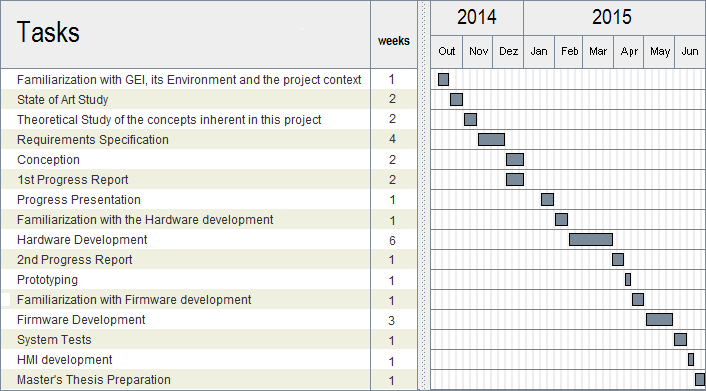
\includegraphics[width=1\textwidth]{Figures/gantt.png}
\caption[Gantt Diagram]{Gantt Diagram of the project.}
\label{fig:Gantt}
\end{figure} %Project Management
% Chapter Template

\chapter{Blood Pressure Measurment} % Main chapter title

\label{Chapter3} % Change X to a consecutive number; for referencing this chapter elsewhere, use \ref{ChapterX}

\lhead{Chapter 3. \emph{Blood Pressure Measurment}} % Change X to a consecutive number; this is for the header on each page - perhaps a shortened title

%----------------------------------------------------------------------------------------
%	SECTION 1
%----------------------------------------------------------------------------------------

why blood pressure measurment is important? most used because

\section{Physiological Process}




Lorem ipsum dolor sit amet, consectetur adipiscing elit. Aliquam ultricies lacinia euismod. Nam tempus risus in dolor rhoncus in interdum enim tincidunt. Donec vel nunc neque. In condimentum ullamcorper quam non consequat. Fusce sagittis tempor feugiat. Fusce magna erat, molestie eu convallis ut, tempus sed arcu. Quisque molestie, ante a tincidunt ullamcorper, sapien enim dignissim lacus, in semper nibh erat lobortis purus. Integer dapibus ligula ac risus convallis pellentesque.

%-----------------------------------
%	SUBSECTION 1
%-----------------------------------
\section{Signal Characteristics}


Onda

Pressão sistolica

Pressão diastolica

Pressão média


Nunc posuere quam at lectus tristique eu ultrices augue venenatis. Vestibulum ante ipsum primis in faucibus orci luctus et ultrices posuere cubilia Curae; Aliquam erat volutpat. Vivamus sodales tortor eget quam adipiscing in vulputate ante ullamcorper. Sed eros ante, lacinia et sollicitudin et, aliquam sit amet augue. In hac habitasse platea dictumst.

\section{Components}

\textbf{Solenoid pneumatic valve}
external diammeter of 3 mm 

\textbf{Pressure Bomb}
external diammeter of 4.3 mm

\textbf{Patient Monitor NIBP connector}
external diammeter of 3,97 mm

\textbf{Pressure Sensor}
external diammeter of 3.04 mm

\textbf{T connector }
external diammeter of 3 mm

\textbf{Optocoupler}

\textbf{Tube}
external diammeter of 4 mm and internal diammeter of 2.5 mm

%-----------------------------------
%	SUBSECTION 2
%-----------------------------------

\section{State of the Art}

The former cenas whilst the latter cenas

Introduction to SoA (numbers)

%----------------------------------------------------------------------------------------
%	SECTION 2
%----------------------------------------------------------------------------------------

\subsection{Litterature}

For over a century the technique of blood pressure measurement developed by Riva-Rocci and Korotkoff has provided most of the data on hypertension diagnosis and treatment. Its limitations, however, are becoming increasingly evident and therefore alternative solutions are under investigation.~\cite{review}

\subsection{Solutions}

Braço

Fixo

Sensitivity etc

Normas de Segurança (Europeias, Americanas, etc)
\subsubsection{One Care Sensing}
One Care Sensing - http://www.onecare.pt/pt/pagina/2/

- ISA não avançou porque o financiamento parou (4 anos), apitava muito/má qualidade (FALAR COM A ISA)

O OneCare Sensing é um kit de fácil utilização que permite monitorizar a tensão arterial, frequência cardíaca, peso e glicemia, no domicílio do utilizador. Oferece ainda a possibilidade
de um prestador de cuidados ou profissionais de saúde acompanharem o estado de saúde do utilizador, à distância, contactando-o sempre que ocorram alterações relevantes nos parametros avaliados[24]. 

Medições são feitas pelo utilizador, no conforto da sua casa e ficam automaticamente disponíveis online no portal OneCare. Freq ajustável, comunicação bluetooth 

Envio de alertas quando ha desvios (registados no portal, SMS ou mail)

GLouzada

\subsubsection{iHealth}
In 2012 iHealth launched the first wireless blood pressure monitor, and in 2013, the first wireless blood glucose monitor. iHealth made the first health devices to be carried in Apple retail stores. Its products are now sold in shops like Walgreens, Best Buy, and Amazon.

25M Xiaomi

\subsubsection{Omron} 

Omron

\subsubsection{Plux BioSignals}
Pressão de Volume Sanguíneo (BVP do inglês Blood Volume Pressure): O sensor de Pressão de Volume Sanguíneo é um sensor ótico não-invasivo que mede variações do volume sanguíneo numa extremidade arterial, baseado na técnica de fotopletismografia. Este sensor possui uma sonda para ser colocada na ponta do dedo com uma fonte de luz vermelha e um fotodetetor. Estes dois componentes estão em modo de deteção de transmissão, e devido à sua configuração permitem assinalar as duas fases do ciclo cardíaco (sístole e diástole). A aplicação mais comum deste tipo de sensor é a medição da frequência cardíaca e da variabilidade de frequência cardíaca.
No entanto, pode ser utilizado para outro tipo de estudos, como a avaliação da




\subsubsection{Software}
iRythm Zio Patch
Convertis AVIVO Mobile Patient Management System
Toumaz SensiumVitals

\section{Overview}

Aplicações: Pacotes de turismo sénior, farmácias, clínicas, lares, IPSS
A table resuming everything %Blood Pressure Measurement
% Chapter Template

\chapter{Acquisition System} % Main chapter title

\label{Chapter4} % Change X to a consecutive number; for referencing this chapter elsewhere, use \ref{ChapterX}

\lhead{Chapter 4. \emph{Acquisition System}} % Change X to a consecutive number; this is for the header on each page - perhaps a shortened title

%----------------------------------------------------------------------------------------
%	SECTION 1
%----------------------------------------------------------------------------------------

\section{YOLO}

Lorem ipsum dolor sit amet, consectetur adipiscing elit. Aliquam ultricies lacinia euismod. Nam tempus risus in dolor rhoncus in interdum enim tincidunt. Donec vel nunc neque. In condimentum ullamcorper quam non consequat. Fusce sagittis tempor feugiat. Fusce magna erat, molestie eu convallis ut, tempus sed arcu. Quisque molestie, ante a tincidunt ullamcorper, sapien enim dignissim lacus, in semper nibh erat lobortis purus. Integer dapibus ligula ac risus convallis pellentesque.

%-----------------------------------
%	SUBSECTION 1
%-----------------------------------
\section{YOLO}

Nunc posuere quam at lectus tristique eu ultrices augue venenatis. Vestibulum ante ipsum primis in faucibus orci luctus et ultrices posuere cubilia Curae; Aliquam erat volutpat. Vivamus sodales tortor eget quam adipiscing in vulputate ante ullamcorper. Sed eros ante, lacinia et sollicitudin et, aliquam sit amet augue. In hac habitasse platea dictumst. %Acquisition System
% Chapter Template

\chapter{Hardware} % Main chapter title

\label{Chapter5} % Change X to a consecutive number; for referencing this chapter elsewhere, use \ref{ChapterX}

\lhead{Chapter 5. \emph{Hardware}} % Change X to a consecutive number; this is for the header on each page - perhaps a shortened title

%----------------------------------------------------------------------------------------
%	SECTION 1
%----------------------------------------------------------------------------------------

\section{YOLO}

Lorem ipsum dolor sit amet, consectetur adipiscing elit. Aliquam ultricies lacinia euismod. Nam tempus risus in dolor rhoncus in interdum enim tincidunt. Donec vel nunc neque. In condimentum ullamcorper quam non consequat. Fusce sagittis tempor feugiat. Fusce magna erat, molestie eu convallis ut, tempus sed arcu. Quisque molestie, ante a tincidunt ullamcorper, sapien enim dignissim lacus, in semper nibh erat lobortis purus. Integer dapibus ligula ac risus convallis pellentesque.

%-----------------------------------
%	SUBSECTION 1
%-----------------------------------
\section{YOLO}

Nunc posuere quam at lectus tristique eu ultrices augue venenatis. Vestibulum ante ipsum primis in faucibus orci luctus et ultrices posuere cubilia Curae; Aliquam erat volutpat. Vivamus sodales tortor eget quam adipiscing in vulputate ante ullamcorper. Sed eros ante, lacinia et sollicitudin et, aliquam sit amet augue. In hac habitasse platea dictumst. %Hardware
% Chapter Template

\chapter{Firmware} % Main chapter title

\label{Chapter6} % Change X to a consecutive number; for referencing this chapter elsewhere, use \ref{ChapterX}

\lhead{Chapter 6. \emph{Firmware}} % Change X to a consecutive number; this is for the header on each page - perhaps a shortened title

%----------------------------------------------------------------------------------------
%	SECTION 1
%----------------------------------------------------------------------------------------

\section{YOLO}

Lorem ipsum dolor sit amet, consectetur adipiscing elit. Aliquam ultricies lacinia euismod. Nam tempus risus in dolor rhoncus in interdum enim tincidunt. Donec vel nunc neque. In condimentum ullamcorper quam non consequat. Fusce sagittis tempor feugiat. Fusce magna erat, molestie eu convallis ut, tempus sed arcu. Quisque molestie, ante a tincidunt ullamcorper, sapien enim dignissim lacus, in semper nibh erat lobortis purus. Integer dapibus ligula ac risus convallis pellentesque.

%-----------------------------------
%	SUBSECTION 1
%-----------------------------------
\section{YOLO}

Nunc posuere quam at lectus tristique eu ultrices augue venenatis. Vestibulum ante ipsum primis in faucibus orci luctus et ultrices posuere cubilia Curae; Aliquam erat volutpat. Vivamus sodales tortor eget quam adipiscing in vulputate ante ullamcorper. Sed eros ante, lacinia et sollicitudin et, aliquam sit amet augue. In hac habitasse platea dictumst. %Firmware
% Chapter Template

\chapter{System Tests} % Main chapter title

\label{Chapter7} % Change X to a consecutive number; for referencing this chapter elsewhere, use \ref{ChapterX}

\lhead{Chapter 7. \emph{System Tests}} % Change X to a consecutive number; this is for the header on each page - perhaps a shortened title

%----------------------------------------------------------------------------------------
%	SECTION 1
%----------------------------------------------------------------------------------------

\section{YOLO}

Lorem ipsum dolor sit amet, consectetur adipiscing elit. Aliquam ultricies lacinia euismod. Nam tempus risus in dolor rhoncus in interdum enim tincidunt. Donec vel nunc neque. In condimentum ullamcorper quam non consequat. Fusce sagittis tempor feugiat. Fusce magna erat, molestie eu convallis ut, tempus sed arcu. Quisque molestie, ante a tincidunt ullamcorper, sapien enim dignissim lacus, in semper nibh erat lobortis purus. Integer dapibus ligula ac risus convallis pellentesque.

%-----------------------------------
%	SUBSECTION 1
%-----------------------------------
\section{YOLO}

Nunc posuere quam at lectus tristique eu ultrices augue venenatis. Vestibulum ante ipsum primis in faucibus orci luctus et ultrices posuere cubilia Curae; Aliquam erat volutpat. Vivamus sodales tortor eget quam adipiscing in vulputate ante ullamcorper. Sed eros ante, lacinia et sollicitudin et, aliquam sit amet augue. In hac habitasse platea dictumst. %System Tests
% Chapter Template

\chapter{Data Storage} % Main chapter title

\label{Chapter8} % Change X to a consecutive number; for referencing this chapter elsewhere, use \ref{ChapterX}

\lhead{Chapter 8. \emph{Data Storage}} % Change X to a consecutive number; this is for the header on each page - perhaps a shortened title

%----------------------------------------------------------------------------------------
%	SECTION 1
%----------------------------------------------------------------------------------------

\section{YOLO}

Lorem ipsum dolor sit amet, consectetur adipiscing elit. Aliquam ultricies lacinia euismod. Nam tempus risus in dolor rhoncus in interdum enim tincidunt. Donec vel nunc neque. In condimentum ullamcorper quam non consequat. Fusce sagittis tempor feugiat. Fusce magna erat, molestie eu convallis ut, tempus sed arcu. Quisque molestie, ante a tincidunt ullamcorper, sapien enim dignissim lacus, in semper nibh erat lobortis purus. Integer dapibus ligula ac risus convallis pellentesque.

%-----------------------------------
%	SUBSECTION 1
%-----------------------------------
\section{YOLO}

Nunc posuere quam at lectus tristique eu ultrices augue venenatis. Vestibulum ante ipsum primis in faucibus orci luctus et ultrices posuere cubilia Curae; Aliquam erat volutpat. Vivamus sodales tortor eget quam adipiscing in vulputate ante ullamcorper. Sed eros ante, lacinia et sollicitudin et, aliquam sit amet augue. In hac habitasse platea dictumst. %Data Storage or Communication
% Chapter Template

\chapter{Conclusion} % Main chapter title

\label{Chapter9} % Change X to a consecutive number; for referencing this chapter elsewhere, use \ref{ChapterX}

\lhead{Chapter 9. \emph{Conclusion}} % Change X to a consecutive number; this is for the header on each page - perhaps a shortened title

%----------------------------------------------------------------------------------------
%	SECTION 1
%----------------------------------------------------------------------------------------

\section{Final Result}

Lorem ipsum dolor sit amet, consectetur adipiscing elit. Aliquam ultricies lacinia euismod. Nam tempus risus in dolor rhoncus in interdum enim tincidunt. Donec vel nunc neque. In condimentum ullamcorper quam non consequat. Fusce sagittis tempor feugiat. Fusce magna erat, molestie eu convallis ut, tempus sed arcu. Quisque molestie, ante a tincidunt ullamcorper, sapien enim dignissim lacus, in semper nibh erat lobortis purus. Integer dapibus ligula ac risus convallis pellentesque.

%-----------------------------------
%	SUBSECTION 1
%-----------------------------------
\section{Future Work}

- minuterize
- portable (I had that in mind when creating the algorithm)
- better system/Big Data (new communication protocol and new data storage) - Tese GLouzada %Conclusion - Final Result, Academic Validation, Market Validation, Future Work



%----------------------------------------------------------------------------------------
%	THESIS CONTENT - APPENDICES
%----------------------------------------------------------------------------------------

\addtocontents{toc}{\vspace{2em}} % Add a gap in the Contents, for aesthetics

\appendix % Cue to tell LaTeX that the following 'chapters' are Appendices

% Include the appendices of the thesis as separate files from the Appendices folder
% Uncomment the lines as you write the Appendices

% Appendix A

\chapter{Appendix Title Here} % Main appendix title

\label{AppendixA} % For referencing this appendix elsewhere, use \ref{AppendixA}

\lhead{Appendix A. \emph{Appendix Title Here}} % This is for the header on each page - perhaps a shortened title

Write your Appendix content here.
%\input{Appendices/AppendixB}
%\input{Appendices/AppendixC}

\addtocontents{toc}{\vspace{2em}} % Add a gap in the Contents, for aesthetics

\backmatter

%----------------------------------------------------------------------------------------
%	BIBLIOGRAPHY
%----------------------------------------------------------------------------------------

\label{Bibliography}

\lhead{\emph{Bibliography}} % Change the page header to say "Bibliography"

\bibliographystyle{unsrtnat} % Use the "unsrtnat" BibTeX style for formatting the Bibliography

\bibliography{Bibliography} % The references (bibliography) information are stored in the file named "Bibliography.bib"

\end{document}  